% Chapter 2
\newcommand{\systemname}[0]{VideoNote}


\chapter{Navigating Lecture Videos} % Chapter title
\label{ch:visualtranscript} % For referencing the chapter elsewhere, use

%----------------------------------------------------------------------------------------
How viewers watch videos depends on the content of the video and the viewers'
needs. For example, watching a film in a theater is a very different experience
from watching a video tutorial on YouTube about how to cook brussel sprouts.
Even for a same video, someone who is watching it for the first time may have a
different approach from someone who has seen the video previously and is
watching again only to review. In this chapter, we focus on the scenario of
watching lecture videos. \\

Lecture videos are growing in popularity, especially through Massive Open Online Courses
(MOOCs) and flipped classroom models.
However, learning with these videos using existing video player interfaces can
be challenging. Viewers cannot digest the lecture material at their
own pace, and it is also difficult to search or skim the content. For these and other
reasons, some viewers prefer lecture notes or textbooks to videos.\\

To address these limitations, we design \textbf{\systemname}, a readable
interface for lecture videos that resmebles lecture notes with figures and text.
\systemname\ combines visuals presented in the lecture
with its transcript text. To generate a \systemname, we first segment the visual content
of a lecture into a set of discrete \emph{visual entities} that correspond to equations, figures, or lines of text. Then, we analyze
the temporal correspondence between the transcript and the visuals to determine their relationships. Finally, based on the inferred relationships, we arrange the text and visuals into a hierarchical and linear layout. \\

We compare our interface with a standard video player, and a state-of-the-art interface designed specifically for 
lecture videos. User evaluation suggests that users prefer \systemname\ for the task of learning and that \systemname\
facilitates browsing and searching in lecture videos.

%----------------------------------------------------------------------------------------

\section{Introduction}
Despite the increasingly important and broad role of lecture videos in education, learning from such videos poses some challenges. 
%
It is difficult for viewers to consume video content at their own pace~\cite{chi2012mixt}.
%
To skip quickly through familiar concepts or slowly review more difficult material, the viewer must interrupt playback and scrub back-and-forth in the timeline.
%
It is also difficult to find specific information in a video. While scrubbing allows users to browse the visual information in the lecture, it is not effective for skimming the audio content, which often includes critical explanations and context that accompany the visuals. As an alternative, some platforms (e.g., Khan Academy and YouTube) provide synchronized transcripts that allow users to click on a phrase and play the video at that location. However, skimming the transcript for relevant content can also be challenging since the text is not structured, and viewers must click on various parts of the text to see the corresponding visuals. 
%
Finally, it is hard to get a quick overview of the lecture content without watching the entire video. 
For these and other reasons, some people prefer static learning materials such as textbooks or printed lecture notes over videos.\\

Inspired by lecture notes, we present \systemname, a readable interface for both the visual and audio content of a lecture video that facilitates reviewing, browsing and navigation. 
%
We focus on blackboard-style lectures that show a (possibly infinite) blackboard where the instructor writes down by hand the content of the lecture. \systemname s aggregate the full lecture content in a structured format where visual information is segmented and grouped with the corresponding narration text. For example, Figure~\ref{Fig:videonote_example} shows our automatically generated output for a math lecture that interleaves verbal explanations with the corresponding equations written on the board. 
%
By default, \systemname s hide redundant information to show a compact representation of the content that viewers can expand interactively to show relevant details (Figure~\ref{Fig:videonote_expanded}). 
%
Presenting video content in this manner allows users to review the lecture at their own pace while getting both the visual and textual information in a readable, skimmable format.
%
\systemname s is also linked to the video such that clicking on the text or the visuals plays the video from the corresponding location.
%
In this respect, \systemname s offer many of the benefits of traditional static media, such as textbooks and lecture notes, while also giving viewers direct access to the video content.\\

There are two main challenges in transforming a video and its transcribed audio into a \systemname : (1) visuals, which are drawn progressively on the board, must be discretized into  a set of meaningful figures, and (2) such figures and text representing the audio content must be organized into a compact, structured format that emphasizes the relationships between the two channels of information.
%
To segment the visuals into meaningful figures, we propose a dynamic programming approach that takes into account both the spatial layout of strokes and the time when they were drawn. We further time-align the transcript with the audio and use this alignment to establish correspondences between the visuals and the text. Finally, we use the visual-text correspondence to detect redundant information and arrange the content in a compact, sequential layout where the text is organized into readable paragraphs.\\

We evaluate our approach with a user study that compares \systemname\ with a baseline transcript-based video player, and an existing, state-of-the-art visual-based video player developed by Monserrat et al \cite{monserrat2013notevideo}. We measure performance on summarization and search tasks, and observe how the participants interact with the interfaces. We find that \systemname\ is an effective interface for studying lecture videos. Specifically, users performed best using \systemname\ for search tasks involving text. Users noted that \systemname\ helped them to get a quick overview of the video including the details conveyed only through the text, and to efficiently focus on parts of interest. They also found the structured text easier to read and connect to relevant visuals than the baseline text-only transcript. In a post-study survey, users strongly preferred our interface for learning over the other two interfaces.\\
%---------------------------------------------------------------------------------------
\begin{figure}[ht!]
        \centering
        \begin{subfigure}[b]{\textwidth}
        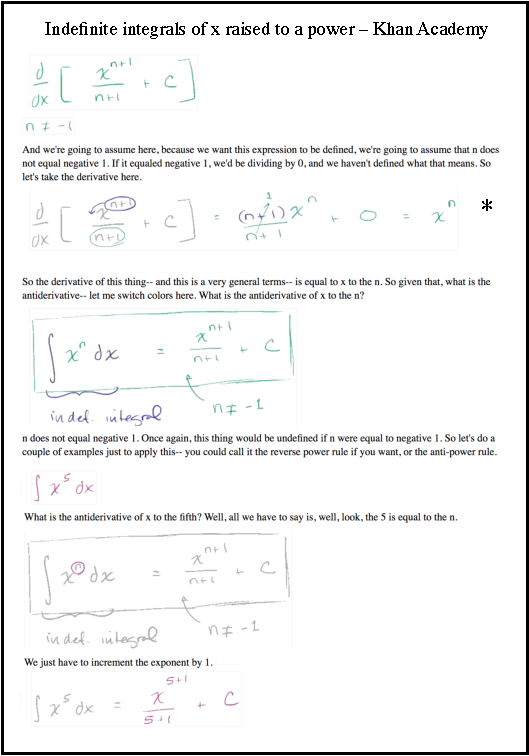
\includegraphics[width=\textwidth]{figures/khan3_page1.pdf}
        \end{subfigure}
        \caption{Example VideoNote}
        \end{figure}
\begin{figure}[!ht]\ContinuedFloat
        \centering
        \begin{subfigure}[b]{\textwidth}
        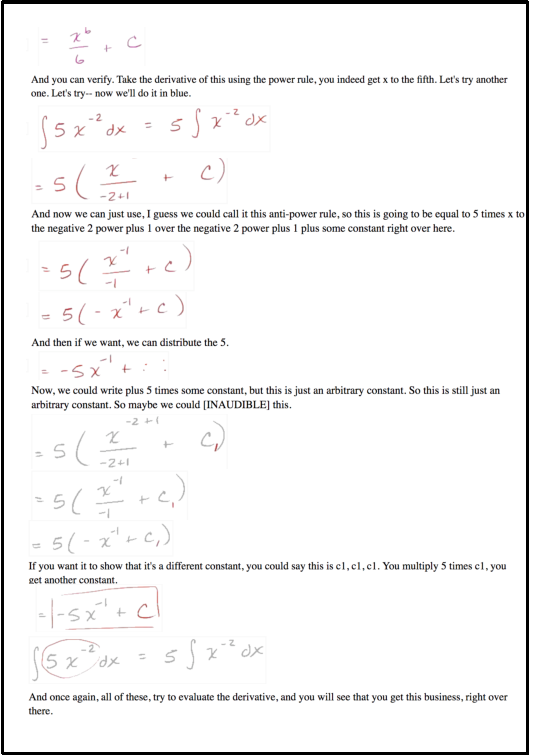
\includegraphics[width=\textwidth]{figures/khan3_page2.pdf}
        \end{subfigure}       
        \caption{Example VideoNote (continued)}
        \label{Fig:videonote_example} 
\end{figure}
%

%----------------------------------------------------------------------------------------
\section{Previous Work}
%
\subsection{Video Visualization}
There is a large body of work that aims to automatically summarize videos to facilitate navigation and browsing, but most research focuses on live action footage which is very different from educational videos.  Recent survey papers \cite{truong2007video,borgo2011survey} comprehensively review these techniques, which can be broadly divided into two classes according to their output: \textit{video skims} and \textit{still-image abstracts}. \\
%
Video skims \cite{he1999auto,ekin2003automatic,ngo2005video,lu2013story} summarize a longer video with a shorter video, usually consisting of segments extracted from the original video. These skims retain audio and motion elements and are especially useful for understanding dynamic scenes, but they are less suitable for conveying the dense, static information of blackboard-style lectures. \\
%
Still-image based methods~\cite{uchihashi1999video,barnes2010video,hwang2006cinema,boreczky2000interactive}
primarily focus on conveying the visual content of a
video in static form through a collection of salient images extracted from the video.~\cite{christel2002collages} and~\cite{pickering2003anses} developed a still-image based method specific to news stories that combines text and images into summaries.\\
%
Most relevant to our work is~\cite{choudary2007summarization}, which summarizes blackboard-style lectures by creating a panoramic frame of the board. In addition to the visual content presented on the board, our interface includes the audio content and therefore maintains the sequence of the lecture and makes textual content directly accessible as well.\\

\subsection{Tools for Online Lecture Videos}
\cite{kim2014data} uses interaction data collected from MOOC platforms to introduce a set of techniques that augment existing video interface widgets. For lecture videos based on slides, \cite{li2000browsing} use separate slides to automatically generate table-of-content overviews. These works \textit{annotate} the original video with useful data to facilitate navigation, but do not reformat the video content. \cite{pavel2014video} provides a tool to create \textit{video digests}, structured summaries of informational videos organized into chapters and sections.\\
%
They use  only the transcript to segment and summarize the video, whereas we leverage both the visual and audio content. Most closely related to our work is Monserrat et al.'s interface \cite{monserrat2013notevideo}, which presents a summary image of blackboard-style lecture videos. Their image is composed of click-able visual links to support spatial and temporal navigation. Although they provide a search box for the transcript, text is not included as part of their summary display.

%----------------------------------------------------------------------------------------
\section{Design Principles}
\label{sec:principles}
%
The design of \systemname\ is informed by the following key characteristics of blackboard-style lectures:
%
\paragraph{Lectures present information progressively.}
Most lectures convey concepts in a progressive manner where each new piece of information builds on the previously presented content.
For example, Figure~\ref{Fig:key_ideas} (\textit{top}) shows a panoramic image of the board for an entire lecture, where the labels show the order in which things were presented. Understanding the lecture often requires knowing this order.
%
To emphasize presentation order, our \systemname\ arranges all the content within the video in a top-to-bottom linear format.
%
\paragraph{Visuals are organized into discrete entities.} The visual content of a lecture is typically organized into well-defined entities (e.g., a line of text, an equation, an explanatory figure) that correspond to the set of presented concepts. 
%
For example, Figure~\ref{Fig:key_ideas} (\textit{top}) shows visual entities in a calculus lecture.   Each visual entity consists of strokes that are close together in both space and time. Moreover, since people are accustomed to parsing visual information line-by-line, from top to bottom, and left to right, visual entities are often laid out in the same manner. 
%
Building on this observation, our system segments drawings on the board into visual entities based on their spatial alignment and temporal proximity.
%
\paragraph{Audio content complements visuals.}
In our analysis of lecture videos, we found that verbal explanations tend to serve one of two broad objectives. Explanations given while the instructor is not drawing are often \emph{explanatory}, providing additional information not directly represented in the visuals or making connections between drawings. On the other hand, explanations given while the instructor is drawing are typically more \emph{depictive}, repeating or reading aloud the visual information (Figure~\ref{Fig:key_ideas}, \textit{bottom}).
%
While depictive explanations can help viewers follow along with the video, they often result in long, repetitive transcript text that is cumbersome to read or skim through. This problem is exacerbated by the fact that most spoken explanations are somewhat colloquial.\\
%
Our interface automatically categorizes transcript text as explanatory or depictive, and in our output, we hide depictive sentences and show explanatory text interspersed with the set of visual entities extracted from the video. 
\cite{large1995multimedia} and \cite{christel2001effect} have shown that such combinations of pictures and captions aid recall and comprehension as well as navigation of video material.
%
Our design gives the viewer relevant context for understanding the visual information without cluttering the output with redundant text. 

%----------------------------------------------------------------------------------------
\section{The \systemname\ Interface}
Based on these observations, we designed \textbf{\systemname}, a readable and printable interface that presents both the visual and audio content of a lecture video. Since \systemname\ contains all of the visual and audio information from the original video, it can be used by itself to study the content. Alternatively, it can be linked to the original lecture video to function as an interactive navigation aid. Similar to Monserrat et al's interface \cite{monserrat2013notevideo}, clicking on a visual entity or a transcript sentence plays the original video at that point in time. As the video is played, the corresponding visual entity and/or transcript sentence is highlighted. \\

Figure ~\ref{fig:examples} shows examples of \systemname\ created from \todo{lecture video}. Please visit \todo{url} for the interactive version of the example. Given an input video and its transcript, we generate \systemname\ automatically using the algorithms described in the next section. To test the robustness of our method, we generated \systemname s of 20 lecture videos from 11 different instructors. Please view the appendix for all the results. Here we highlight some of the key features of \systemname .\\
%
\paragraph{Linear format highlights lecture progression.} The layout of text and visual entities in \systemname\ often emphasizes the instructor's thought process and clarifies the intermediate steps that lead to a result. Figure~\ref{Fig:feature_highlight}~(left) compares equations in the final view of the blackboard at the end of the lecture to our \systemname . Although the blackboard view shows the same set of equations, it is difficult to infer how the equations relate to and build upon each other. Our \systemname\ shows a step-by-step progression of the visual content. 
%
\paragraph{Interspersing text with visuals clarifies connections.} A purely visual summary of the video omits verbal explanations, whereas a purely textual summary (i.e., standard transcript) can be confusing without the corresponding visuals. Instead, \systemname\ interleaves explanatory text and visual entities. This makes it easy to see the connection between illustrations, or the context of an illustration. For instance, compare the leftmost example in Figure~\ref{Fig:visual_line_output}, which shows a final view of the blackboard and Figure \ref{Fig:feature_highlight}~(right) the \systemname\ for the same video. In the former, it is difficult to see the connection between the illustration (pink highlight) and the equation to its right (green highlight) without listening to the lecture. In the latter, the text in-between explains clearly that the equation represents the vector field depicted in the illustration.
%
\begin{figure}[h!]
        \centering
        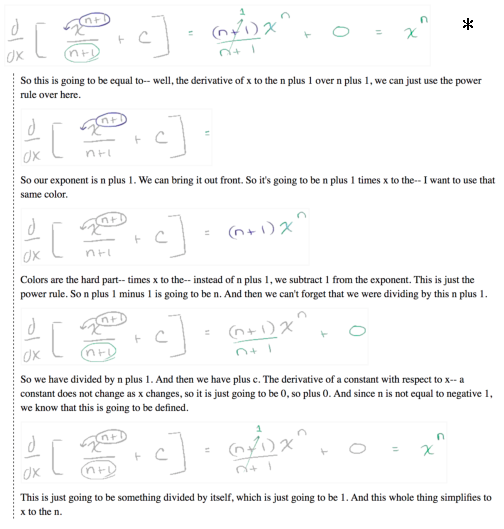
\includegraphics[width=0.8\textwidth]{figures/videonote_expand.pdf}
	\captionsetup{font=footnotesize}
        \caption{\systemname\ is organized hierarchically. The default view hides descriptive details to present a compact summary. Users can click on a higher-level figure to expand its detailed description and step-by-step derivation.} 
        \label{Fig:videonote_expanded}
\end{figure}\\
%
\paragraph{Different levels of detail.} By default, \systemname\ hides redundant depictive text that just describes the corresponding visuals. If a reader wants to see more details, she can reveal the hidden text by clicking on the visual entity. In the case of a long equation or a complicated illustration, the expanded view breaks up the visual and textual information 
into easy-to-read blocks (Figure~\ref{Fig:videonote_expanded}). 
%----------------------------------------------------------------------------------------

\section{Algorithms}
There are three main steps to create \systemname . First, we
segment the visual content of a lecture into visual entities using a
dynamic programming approach (\ref{sec:segmentation}). Then, we 
structure the transcript content by computing temporal correspondences
between visual entities and transcript sentences
(\ref{sec:text_corr}). Finally, we generate a \systemname\ by interleaving visual entities with transcript text (\ref{sec:layout}). The rest of this section describes each of these steps in detail.
%
\subsection{Pre-processing}
The visual content in blackboard-style lectures consists of \emph{strokes},
the set of foreground pixels generated during one continuous drawing action.
In the context of a graphics tablet, a stroke corresponds to the continuous
path of a pen while maintaining contact with the writing surface. \todo{Explain that this is not exactly the case in our pre-processing step.} As a pre-processing step, we extract
individual strokes from the input video using a method similar to
\cite{monserrat2013notevideo}.  We detect the start and end time of
each drawing action by comparing the number of foreground pixels in
consecutive frames. A large increase marks the start of an action,
while no change marks the end. The difference image between the end
and start frames gives an image of the stroke drawn during that
period.
The manual steps involved in this process are (1) identifying the cursor image, which is automatically removed from all frames, (2) setting a threshold for foreground/background separation, and (3)  setting a smoothing window to get rid of the noise in the foreground pixel count. Depending on the instructor's writing speed, a typical stroke
comprises several characters to several words, or it can also be a
part of an illustration or a graph (Figure~\ref{Fig:stroke_examples}).\\

In addition
to the visuals, lecture videos include an audio track with the instructor's
spoken explanations. Several on-line video lecture platforms (e.g. Khan Academy,
YouTube) provide transcripts of the audio. We assume such transcripts and
we use an online audio transcription service (\url{castingwords.com}) if they are
not available. 
%
\subsection{Segmenting Visual Content}
\label{sec:segmentation}
One straightforward strategy for grouping strokes into visual entities
is to process strokes in the order they are drawn and decide whether
each stroke represents the start of a new visual entity or is part of
an existing visual entity formed by previous strokes \cite{mynatt1999flatland}.
While this simple, greedy approach works in some cases, there are many
scenarios where it leads to poor segmentations. 
\marginpar{
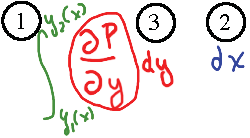
\includegraphics[width=1.2in]{figures/greedy_ex-2.pdf}
\captionsetup{font=footnotesize}
 \captionof{figure}{Without considering the semantics of these symbols and before the last stroke ($\frac{\delta p}{\delta y}dy$) is inserted, the first two strokes ($-\int^a_b$ and $dx$) appear like two separate equations with a large space between them.}
\label{fig:baselineinset}
}
For example, in
Figure~\ref{fig:baselineinset}, there is a large space between the first stroke ($-\int^a_b$, \raisebox{.5pt}{\textcircled{\raisebox{-.9pt} {1}}}) and the second stroke ($dx$, \raisebox{.5pt}{\textcircled{\raisebox{-.9pt} {2}}}). Without considering the semantics of these symbols, 
they appear to be separate equations. However, once we consider 
the subsequent set of red strokes(\raisebox{.5pt}{\textcircled{\raisebox{-.9pt} {3}}})
 it becomes clear that this is not the best segmentation. In general, computing good stroke segmentations requires considering
the global configuration of strokes in both space and time. \\

In this respect, the problem of segmenting strokes into visual
entities is analogous to the
\emph{line-breaking} problem, i.e., arranging the words of a paragraph
into lines.  In both cases, we want to segment a sequence of elements
(strokes or words) into an optimal set of groups (visual entities or
lines) defined by some scoring function over candidate entities or lines.
An important difference is that in the traditional line-breaking problem, only a
contiguous set of words can be put on the same line. In our case,
strokes in one visual entity can be interspersed by strokes in a
different visual entity. For example, the instructor may
go back and forth between two lines of equations, or
between a graph and an equation (Figure~\ref{Fig:line_order}).\\

Given these observations, we propose a dynamic programming approach for
stroke segmentation based on the classic optimal line-breaking
algorithm~\cite{knuth1981breaking} that handles non-contiguous grouping.
We first explain the high-level structure of the algorithm before
describing the scoring function in deta
%
\subsubsection{Algorithm Overview}
Figure \ref{Fig:pseudocode} gives a detailed pseudo-code of our segmentation algorithm.\\    
%
\begin{figure}[h!]
        \centering
        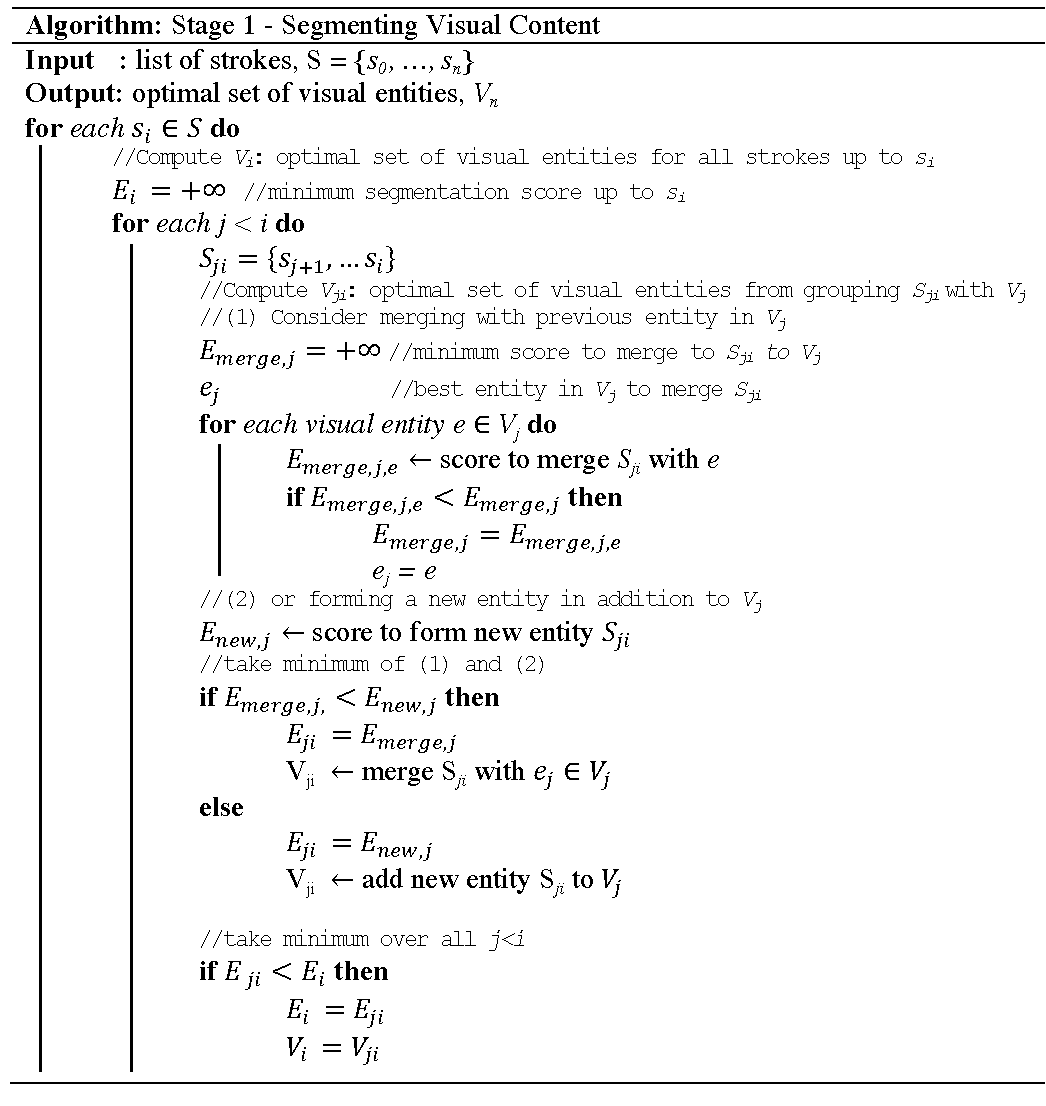
\includegraphics[width=\textwidth]{figures/pseudocode_image.pdf}
	\captionsetup{font=footnotesize}
        \caption{We use dynamic programming to segment strokes into an optimal
set of visual entities. For each stroke, $s_i$, the algorithm considers all previous
partial solutions, $V_{j<i}$ and $S_{ji}=\{s_{j+1}, ..., s_i\}$. For each
$V_j$, it considers two possibilities: merging $S_{ji}$ with an existing
entity or forming a new entity.}
        \label{Fig:pseudocode}
\end{figure}\\
%
Given a sequence of $n$ strokes $S = \{s_o,\dots,s_n\}$ ordered by
when they appear in the video, we find the optimal set of inter-stroke
boundaries that segment the strokes into visual entities. We refer to the boundary between $s_i$ and $s_{i+1}$ as
$b_i$.
%
Our algorithm processes the strokes in order and for each $s_i$
computes and records the optimal set of visual entities $V_i$ formed
by all strokes up to $b_i$, along with the total score $E(V_i)$ of
this partial solution.
%
To determine the optimal partial solution for stroke $s_i$, we
consider each previous boundary $b_j$ where
$\setlength{\thickmuskip}{0mu} j<i$, and evaluate two possible ways of
grouping the set of strokes $S_{ji} = \{s_\text{j+1},
\dots,s_\text{i}\}$: 1) merging $S_{ji}$ with one of the existing entities
in $V_j$, or 2) forming a new entity with $S_{ji}$. 
%
Allowing $S_{ji}$ to be merged with existing entities enables our
algorithm to support non-contiguous stroke groupings.
%
We take the better (lower) of the two scores for $S_{ji}$ and add it
to $E(V_j)$ to obtain the total score for the proposed
segmentation. After considering all candidate boundaries $b_j$, we
identify the partial solution with the minimum segmentation score and
record the corresponding set of entities as $V_i$ and the score as $E(V_i)$.
%
Once the algorithm iterates through all strokes, $V_n$ gives the
optimal set of visual entities for the entire lecture.
%
%
\subsubsection{Scoring Function}
The dynamic programming algorithm described above requires a scoring
function that evaluates the goodness of candidate visual entities
formed by sets of strokes. We define this scoring function based on
several observations: Strokes within a visual entity are (1) compactly arranged (2) and horizontally aligned. In addition, separate visual entities are (3) spatio-temporally distant from each other.
%
\paragraph{(1) Visual entities are compact.} Strokes that belong together
in the same visual entity are typically arranged in a compact way. We
consider two measures of compactness for a visual line:
horizontal and vertical.

\begin{figure}[h!]
	\centering
        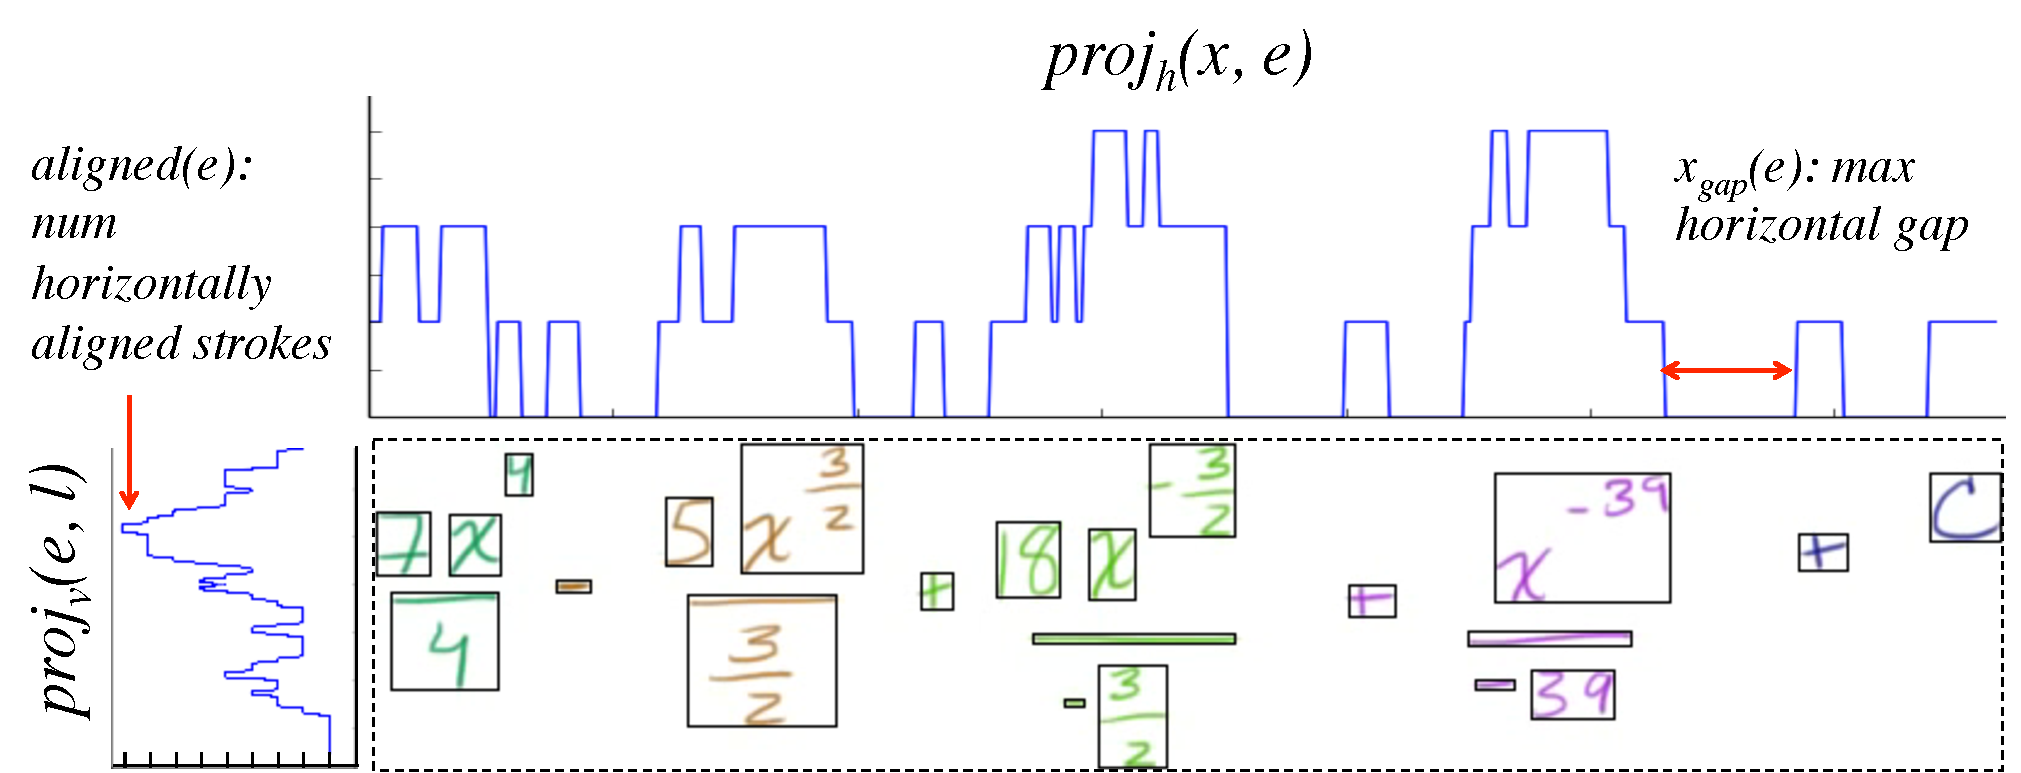
\includegraphics[width=\textwidth]{figures/projection_function.pdf}
        	\captionsetup{font=footnotesize}
        \caption{Horizontal ($proj_h$) and vertical ($proj_v$) projection functions of strokes in a line. In this example, $y_\text{gap}(e)=0$.}
        \label{Fig:projection_function}
\end{figure}

\begin{itemize}
\item \textbf{Horizontal Compactness:} Intuitively, horizontal compactness is related to the horizontal
\emph{gap} between strokes within a visual entity. Figure \ref{Fig:projection_function}
shows an illustration of how gaps between strokes are measured. First, we define a horizontal projection function for a set of strokes, $S$, as 
\begin{equation}
proj_h(x, S) = \big{|}\{s\in S \small{|} x_\text{min}(s)\le x \le x_\text{max}(s)\}\big{|}
\label{Eq:projh}
\end{equation}\\  
where $x_\text{min}(s)$, and $x_\text{max}(s)$ are the minimum and maximum $x$-coordinates of the bounding box of stroke $s$ respectively. Then, the maximum horizontal gap of a visual entity $e$ is
 \begin{equation}
 x_\text{gap}(e) = \argmax_{x_i, x_\text{i+1}} (x_\text{i+1}
 - x_i)
 \end{equation}
where $x_i$ and $x_\text{i+1}$ are distinct consecutive elements in the ordered set $X =\{\,x \mid proj_{h}(x,e)\ne 0\,\} $. We observed that the horizontal gap between different visual entities
is usually around 100 pixels or more, so we define a horizontal compactness
term $C_{h}$ that imposes harsher penalties when the maximum
horizontal gap exceeds this distance.
\begin{equation}
C_{h}(e) = \big(\frac{x_\text{gap}(e)}{100}\big)^2
\end{equation}

\item \textbf{Vertical Compactness:} Vertical compactness is defined similarly in terms of a vertical projection
function, $proj_{v}$, the maximum vertical gap,
$y_\text{gap}(e)$, and a typical vertical gap of 40 pixels between
different visual entities.
\begin{equation}
C_v(e) = \big(\frac{y_\text{gap}(e)}{40}\big)^2
\end{equation}
\end{itemize}

\paragraph{(2) Strokes within a visual entity are aligned horizontally.} With the exception
of certain illustrations such as graphs, the strokes in most visual
entities are horizontally aligned (e.g., equations, lines of
text). Thus, we prefer to group horizontally aligned strokes into a single
entity. The number of horizontally aligned strokes in each visual entity is computed by taking the mode of its vertical projection function (Figure \ref{Fig:projection_function}).
\begin{equation}
aligned(e) = \argmax_{y_\text{min}(e) \le y \le y_\text{max}(e)} proj_v(y)
\end{equation}
We then define an alignment term $C_a$ whose contribution gradually
diminishes with the total number of aligned strokes.
\begin{equation}
C_a(e) = aligned(e)-\frac{1}{aligned(e)+1}
\label{Eq:n_align}
\end{equation}

\begin{figure}[h!]
        \centering
        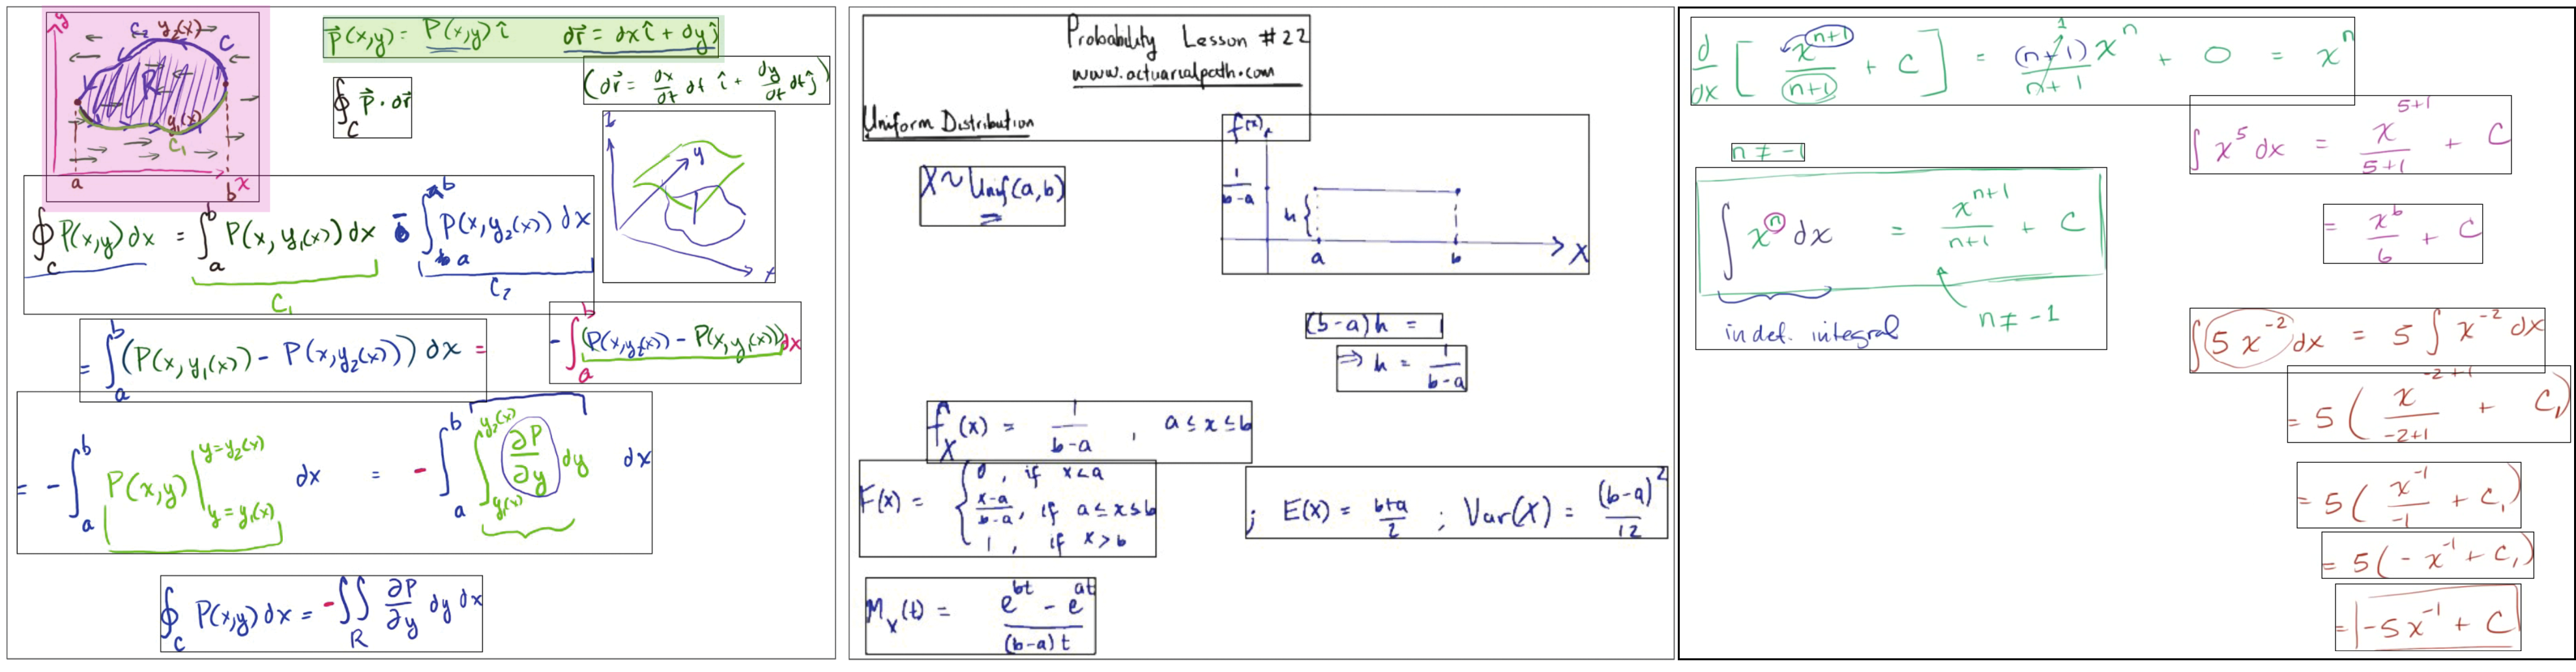
\includegraphics[width=\textwidth]{figures/visual-lines2.pdf}
        \captionsetup{font=footnotesize}
        \caption{Examples of visual entities output from our line-breaking algorithm.
Our algorithm successfully identifies meaningful groups even from complex
layouts with a mix of equations, figures and graphs.}
        \label{Fig:visual_line_output}
\end{figure}

\paragraph{(3) Visual entities are spatio-temporally distant from each other.} This observation
is complementary to the first observation, i.e. visual entities are
compact. Whereas strokes that belong together are written close
together, instructors usually leave some space on the board, for
example, between lines of equations or separate illustrations. We
express this property by penalizing any overlap between distinct
visual entities, measured by the overlapping
area between their bounding boxes. In particular, we define the overlap
penalty term
\begin{equation}
P_{o}(V) = \sum_{e_i,e_j \in V, i \neq j}\big(\frac{area(e_i\cap e_j)}{min(area(e_i), area(e_j))}\big)
\label{Eq:overlap_penalty}
\end{equation}
A similar property holds in the temporal domain. For example, after
writing a single line of an equation and before going on to the next
line, there is a brief pause while the instructor moves the cursor to
the next position or provides some verbal explanation. We compute the
temporal distance between two consecutive strokes across visual entity
boundaries.
\[
    t_\text{dist}(s_i, s_\text{i+1})= 
\begin{cases}
   0, \text{if } s_i, s_\text{i+1 } \text{belong to the same visual entity}\\
   start(s_\text{i+1}) - end(s_i), \text{otherwise}
\end{cases}
\]
where $start(\cdot)$ and $end(\cdot)$ are the start and end times of
when a stroke is drawn in the video. We penalize visual entity
boundaries with a small temporal gap.
\begin{equation}
P_{t}(V) = \sum_{i = 0}^{n-1}\frac{1}{t_\text{dist}(s_i, s_{i+1})}
\end{equation}
where $n$ is the total number of strokes.\\

\paragraph{Combining scoring terms.} So far, we have defined terms that measure the compactness ($C_h, C_v$) and horizontal alignment ($C_a$) of an individual visual entity $e$, as well as the spatio-temporal distance ($P_o, P_t$) between a set of candidate entities $V$. 
%
We combine all these terms into a single scoring function $F$ as follows.  
\begin{align}
F(V) = &\sum_{e \in V}[C_v(e) + 0.5C_h(e)- C_a(e)]&\\
&+ P_o(V) + P_t(V)
\end{align}\\
The factor of 0.5 puts a smaller weight on horizontal versus vertical
gaps. Higher values of $C_a$ indicate more horizontally aligned strokes and better segmentation, so we put a minus in front.\\

The final output of our algorithm is a grouping of all the strokes on the
board into a set of meaningful visual entities (Figure~\ref{Fig:visual_line_output}).
To test the robustness of our segmentation algorithm, we applied it to 20 video lectures from 10 different authors, using the same set of parameters as described above. The lectures included non-linear layouts of visual content and examples of complex diagrams with several layers of information. In all cases, the algorithm produced reasonable segmentations which generated comprehensible \systemname. There were few cases ($\approx 5\%$) where the output segmentation was less than ideal, but these did not affect the overall quality of the \systemname s. Please see section~\ref{sec:discussion} for more details. The full set of results are included in the appendix. 
%---------------------------------------------------
\subsection{Structuring Transcript Content}
\label{sec:text_corr}

Once we have segmented the visual content of the lecture, the next step is to organize the transcript text with respect to the extracted visual entities.
We leverage temporal correspondences between the transcript and visuals to distinguish between explanatory and depictive sentences (section~\ref{sec:principles}) and to break long text descriptions into shorter, more readable paragraphs.

\subsubsection{Aligning transcript to video.} 
To obtain the temporal alignment between the transcript and video, we use an automatic algorithm by \cite{rubin2013content} which extends the Penn Phonetics Lab Forced Aligner (P2FA) built on the HTK speech recognition software. This   aligner takes a verbatim transcript and an audio file as inputs and outputs a time-stamped transcript, where each word is annotated with a start and end time. 

\subsubsection{Detecting explanatory versus depictive sentences.} 
As discussed in section~\ref{sec:principles} about design principles, depictive sentences typically coincide with drawing actions while explanatory sentences do not. Using the time-aligned transcript,
we compute correspondences between transcript sentences and visual entities.
A sentence is matched to a single visual entity if most of its utterance
time ($ \geq 75\% $) overlaps with the drawing time of the visual entity.
If a sentence does not coincide with any entity, we refer to it as an unmatched
sentence. We classify all matched sentences as depictive text (associated with the corresponding visual entities) and all unmatched sentences as explanatory text.
%
Note that while this is a heuristic, we found it to work well in practice. 
%
We use this information in the layout stage to reduce clutter and make the text more readable.    

\subsubsection{Breaking up long text descriptions.}
%
In some cases, complex visual entities that contain a lot of information may get matched with large blocks of depictive text.
%
When reading such text blocks, it can be hard to identify and follow all the correspondences between the individual sentences and the relevant parts of the figure.
%
We address this problem by breaking up complex visual entities into sub-entities, each of which has a shorter, more readable block of depictive text.\\

In particular, we use a variant of the stroke segmentation algorithm described in the previous section to further segment a complex visual entity $e$.
%
In this case, we use the following scoring function $F_\text{sub}$ to evaluate a set of candidate sub-entities, $V_\text{sub}$:
%
\begin{equation} F_\text{sub}(V_\text{sub}) = \sum_{e_\text{sub} \in V_\text{sub}}\lambda_{1}\lvert n_\text{words}(e_\text{sub}) - w \rvert + P_\text{o}(V_\text{sub}) \end{equation} 
%
where $n_\text{words}(e_\text{sub})$ is the number of words in the depictive text associated with sub-entity, $e_\text{sub}$; $P_\text{o}$ is the overlap between bounding boxes of sub-entities in $V_\text{sub}$ (defined in Equation \ref{Eq:overlap_penalty}); $w$ is the target number of words in the depictive text for each sub-entity; and $\lambda_{1}$ determines the relative importance of the word count and overlap terms. We set $w = 50$ (about 2-4 sentences) and $\lambda_{1} = 1/25$.\\

Using this scoring function, we apply the same dynamic programming procedure described in section~\ref{sec:segmentation} to segment $e$ into sub-entities. In this variant, we only allow consecutive strokes to be grouped together since our goal is to obtain temporally sequential sub-entities.
%
\todo{Figure} shows an example output from this optimization.  
%-----------------------------------
\subsection{Layout and Formatting}
\label{sec:layout}
We organize the visual and audio content into a static, sequential format by interleaving visual entities with blocks of transcript text in the order of their appearance in the video. As we point out in section \ref{sec:segmentation}, a single visual entity can be composed of non-contiguous groups of strokes. For example, in Figure~\ref{Fig:line_order}, $e_1$ and $e_2$ each consist of 4 separate groups of strokes, (1\&2, 4, 6, 8) and (3, 5, 7, 9) respectively. In this case, we show each contiguous group of strokes at its associated time, together with previous strokes in the same visual entity which are shown for context. So Figure~\ref{Fig:line_order} would be presented as: 1\&2, 3, (1\&2)\&4, (3)\&5 etc., where the parentheses indicate previous strokes. The new group of strokes is highlighted with color on top of the previous strokes (Figure~\ref{Fig:layout_line_order}). 
\begin{figure}[h!]
        \centering
        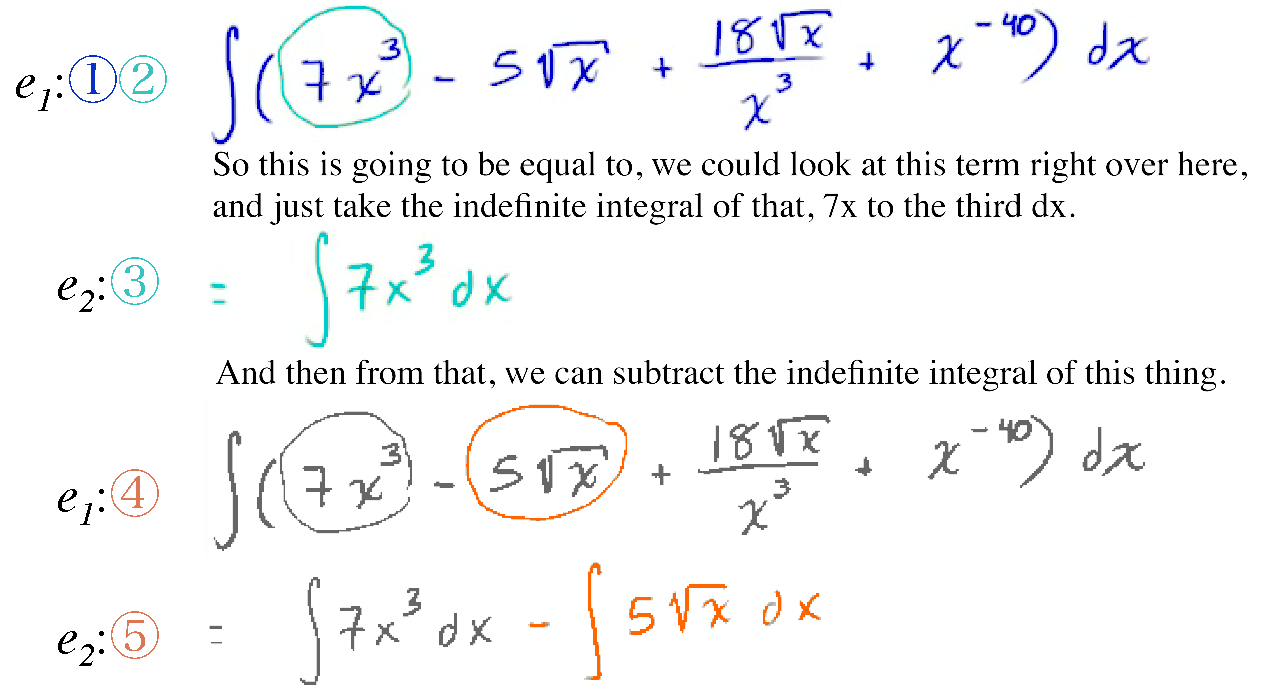
\includegraphics[width=\textwidth]{figures/layout_line_order.pdf}
        \captionsetup{font=footnotesize}
        \caption{\systemname\ presentation of strokes 1-5 of Figure~\ref{Fig:line_order}. Each contiguous group of strokes is shown together with previous strokes in the same visual entity.}
        \label{Fig:layout_line_order}
\end{figure}\\

By default, all visual entities and explanatory sentences are shown; the depictive text associated with visual entities is hidden to reduce clutter. Users can click on the \emph{expand} buttons next to individual visual entities to display the corresponding depictive sentences. For complex visual entities, the expanded view shows the decomposed sub-entities with their associated depictive sentences (Figure~\ref{Fig:teaser}c).\\

%----------------------------------------------------------------------------------------
\section{User Evaluation}
We performed a comparative study to test the hypothesis that \systemname\ facilitates learning. We compared three interfaces to study video lectures: a standard YouTube player with an interactive text transcript (Baseline), Monserrat et al.'s interface \cite{monserrat2013notevideo} (hereafter referred to as \emph{Monserrat}), and our \systemname\ interface linked to the video (Figure~\ref{Fig:interfaces}). The YouTube video player is currently the most common viewing interface for online lectures, and \textit{Monserrat} while less established, was specifically designed to facilitate navigation of blackboard-style lecture videos. In \emph{Monserrat}, a panoramic image of the board with strokes from the entire lecture serves as an in-scene navigation interface. Users can click on any stroke to play the video at that point in time.
%
\subsection {User Tasks}
Our study includes two tasks: (1) summarization, to get a quick and comprehensive overview of the lecture without watching the entire video, and (2) search, to quickly locate specific information.
Although not a direct measure of learning, these tasks are inherent activities in learning and also match common evaluation tasks used in the literature on tools for lecture videos \cite{kim2014data,pavel2014video,monserrat2013notevideo}.\\
%
\begin{description}
\item[Summarization Task]: Users were asked to quickly provide an overview of the lecture without watching the entire video. We gave users only 3 minutes to view and summarize 7-8 minute long lectures. We purposely did not give enough time to watch the entire video so as to motivate the users to quickly scan through its content. Before the task, users watched a sample lecture video and read a sample summary comprised of main points and detail points. Users were encouraged to try to write down at least all the main points of the lecture, and as many of the detail points as possible.\\
%
We compared the summaries written by users to a \text{gold standard} list of main/detail points manually created by two referees. The user summaries were scored by the number of points they covered.
%
\item[Search Task:] The search task emulates scenarios when the user wants to quickly find a specific piece of information in the video (e.g. to solve a question in a problem set, or to look up a specific formula). We differentiate three different types of search problems 
depending on whether the information is in the visuals, the transcript or a combination of both.\\ 
The \textbf{visual search} reproduces situations when a user remembers something visually and wants to find where it appeared. (E.g., \textit{Find the point in the lecture where the instructor strikes out part of an equation, where terms add up to eliminate each other.}) For the \textbf{textual search}, the cue is often a word or a phrase that could be found in the transcript either directly or indirectly (E.g., \textit{Find the point in the lecture where the property that every continuous function has an antiderivative is stated.}) For the \textbf{contextual search}, the information is neither in the text nor visuals alone, but rather in the context between the two. (E.g., \textit{Find the point in the lecture where the instructor writes an integral expression for a bounded area under some curve.})\\
User performance was assessed by the task completion time as well as correctness.
\end{description}

Nine participants (2 female, 7 males), ages 20 to 35 took part in our study. 
All of them were familiar with the general subject matter of the lectures, although they had not seen the particular lectures before.\\
%
We chose three college-level math lectures for our study: \textit{Fundamental Theorem of Calculus} by Salman Khan (8 minutes), \textit{Proving Trigonometry Formulas Using Euler's Formula} by Lee Stemkoski (7.2 minutes), and \textit{Uniform Distribution} by Actuarialpath (8 minutes).\\
We used a within-participant design, where each participant performed tasks on each interface. We counter-balanced the order of the interfaces and the assignment of videos to interfaces using a Latin Square.\\
Before using each interface, participants were briefed about their features and given time to familiarize themselves. After each task, they answered questions about their interaction with the interface. After completing all tasks, participants completed a questionnaire on their preference and the usability of each interface. Please refer to the supplementary material for the full set of tasks and post-task questionnaires.
%--------------------------------------
\subsection{Findings and Discussion}
There are several notable findings from our user study:

\paragraph{(1) Users write more comprehensive summaries with \systemname .}
Users listed the most number of main and detail points using our interface,
although differences across the interfaces were not statistically significant
according to the one-way analysis of variance (ANOVA) (main points:
$F_{2,24}=0.23$, $p=0.79$, detail points: $F_{2,24}=0.48$, $p=0.62$). Table~\ref{Tab:summary_results} shows the percentage of main/detail
points covered by user summaries with each interface.

\begin{table}[!h]
 \centering
 \begin{tabular}{ l |c c c}
 \hline
    & \textbf{Baseline} & \textbf{\textit{Monserrat}} & \textbf{Ours} \\\hline
   \textbf{Main points} & 0.83$\pm0.12$ & 0.81$\pm0.21$ & 0.87$\pm0.18$\\
   \textbf{Detail points} & 0.50$\pm0.22$ & 0.56$\pm0.18$ & 0.58$\pm0.15$\\
   \hline
 \end{tabular}
 \caption{Percentage of points covered by user summaries compared to the
golden standard list.}
 \label{Tab:summary_results}
\end{table}

Note that while on average, there may not seem to be a significant difference
between ours and the two alternatives, summary quality varied
significantly depending on the video. In particular, when the sequence of lecture was not clear in the panoramic image, \textit{Monserrat} users mixed the order of points or missed a main point entirely. For example, in the lecture on \textit{Fundamental Theorem of Calculus} (Figure~\ref{Fig:key_ideas}), \textit{Monserrat} users immediately clicked on the ``Fundamental Theorem'' (\raisebox{.5pt}{\textcircled{\raisebox{-.9pt} {4}}}) skipping the first third of the lecture about the graph of a continuous function and the area under it (\raisebox{.5pt}{\textcircled{\raisebox{-.9pt}
{1}}}-\raisebox{.5pt}{\textcircled{\raisebox{-.9pt}
{3}}}). While users performed comparably with Ours or the baseline, when asked which interface they preferred for the summary task, they preferred \textit{Monserrat} (5/9) and ours (4/9). 

\paragraph{(2) Users find information involving text faster with \systemname\ than with \emph{Monserrat} or the baseline.}
For the \textit{text search} and  the \textit{contextual search} users performed fastest with \systemname\  followed by \textit{Monserrat} and then the baseline (Figure~\ref{Fig:interfaces}, \textit{right}), although the differences across the interfaces were not statistically significant according to the non-parametric Kruskal-Wallis Test ($\chi^2=0.82$,
$p=0.676$).\\ 
For these tasks, users either had to find relevant text or find a visual and also look at the text around it (or listen to the audio). \systemname\ naturally supports such tasks by  interleaving text and figures. \textit{Monserrat} does not provide a text to skim through, but users could search for key words or phrases (a feature also provided in \systemname\ and the baseline). Alternatively, they could click on a visual and listen. Interestingly, the baseline performed worst on these tasks, despite the fact that it is most text-centered and  provides the exact same text as \systemname . This is likely because the text in the baseline was unstructured and difficult to read (see finding 3).\\
For the \textit{visual search} users performed fastest with \textit{Monserrat}. For
all videos we tested, \textit{Monserrat} had the advantage of presenting all the visuals
in one screen, which made it easier for users to scan the entire visual content
without having to scroll.\\
On average, participants' performance on the search task was comparable on
ours and \textit{Monserrat}, which was better than the baseline. The difference between
ours and the baseline was statistically significant with the Mann-Whitney
U (MWU) test ($Z=-2.1$, $p=0.02$), whereas the difference between ours and
\textit{Monserrat} was not ($Z=1.2$, $p=0.12$). Occasionally, users missed the information in their first search attempt and  then tried to scan the entire lecture, contributing to a large variance.  \\
In terms of accuracy, users were most successful in locating the correct information with \systemname\ (average error rate $e=0.06$) compared to \textit{Monserrat} ($e=0.07$) or the baseline ($0.15$), although the differences were not statistically significant (ANOVA, $F_{2,24}=1.04$, $p=0.15$).

\paragraph{(3) \systemname\ makes the transcript text easy to read and skim through.}
Both the baseline and \systemname\ include the entire transcript text. However,
the usefulness of their transcripts is rated very differently. On a 1-7 usefulness
scale, \systemname\ scored 6.3 (range: 5 to 7), whereas baseline scored 4.7
(range: 1 to 7). With the baseline, participants mostly scrubbed
through the timeline to complete the tasks. Several users (3/9) mentioned
that the baseline transcript text was difficult to skim through or find correspondences
with the video. In contrast, with \systemname, users primarily relied on
the text and visuals to solve the tasks (rather than the video). One user
commented that the layout was \textit{``similar to a textbook''} and \textit{``easy
to read''}. Another user said that \textit{``the paragraph structure corresponds
to the main points''} which facilitates skimming.

\paragraph{(4) Users prefer \systemname\ for learning.}
The post-task survey showed that, for learning in general, most users (7/9) preferred our interface over \textit{Monserrat} (2/9) or the baseline. 
The reasons for preferring \systemname\ included \textit{``having the whole script and equations [visuals]''} and \textit{``a good balance between getting the overview and some more detail.''} Those who preferred \textit{Monserrat} appreciated having all visual content presented \textit{at once} without having to scroll, but also noted that the sequence was not apparent (e.g., many users asked where to click to get to the beginning of the lecture) and that \textit{``there's a risk of missing something that's not written on the board.''}\\
%----------------------------------------------------------------------------------------
\section{Discussion}
\label{sec:discussion}
\subsection{Limitations}
\systemname\ focused on blackboard-style lectures, but the key ideas behind the design of \systemname\ (e.g., presenting discrete visual entities next to its corresponding narrative in a linear layout) are generalizable to other style of lecture videos. Different styles of lecture videos would require different or more sophisticated visual entity recognition and layout techniques. For example, a classroom recording might have human occlusion, and a slide-based presentation could have animation or other multimedia effects.\\

The pre-processing step for stroke extraction works especially well with digital blackboard-style lectures with constant background and minimal occlusion. However, videos with more noise (e.g., from lighting change or occlusion by hand) may require a more sophisticated method. We also do not handle special cases
such as partial erasure or copy-and-paste.  For instance, if the instructor
updates a part of visual content in order to correct a mistake, the current
implementation only shows the \textit{newest} stroke.\\

Although in all of our examples the segmentation algorithm outputs produce a comprehensible \systemname\, we also observed 2 types of failure cases: (1) \textit{under-segmentation}, where too many strokes are grouped into a single visual entity, and (2) \textit{over-segmentation}, where related strokes are separated into different visual entities. Our scoring function assumes a layout where distinct visual entities are more or less spatially separate from each other. A different method may be required to handle videos that violate this assumption, for example a history lecture where most of the writing is on top of a map, or where figures are overlayed on top of each other (Figure~\ref{fig:humanities_lec}).  An editing or annotation mechanism, including crowdsourcing, to aid segmentation would be useful and a potential area for future work.\\

In placing temporally aligned visuals and sentences next to each other, we assume that instructors talk about what they are drawing at the same time. This assumption holds in most cases, but fails to resolve other types of references. For example, in Figure\ref{fig:gesture}, the pronoun `here' is used twice, each time referring to a different part of the visual. Whereas in the video these references become clear with the cursor movement, they remain ambiguous in our static output.

%\begin{figure}[t!]
%        \centering
%        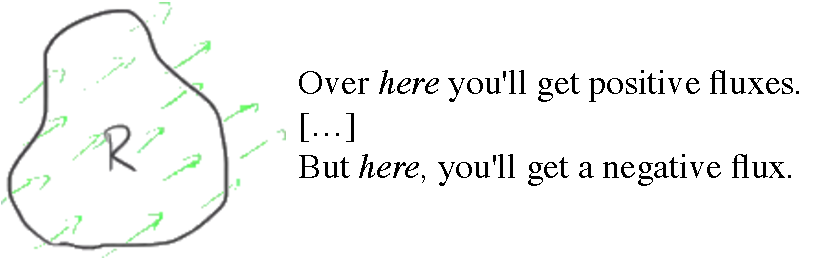
\includegraphics[width=\textwidth]{images/gesture.pdf}
%        \caption{\VEDIT{Layout using only temporal correspondence fails to resolve some references. In this example, `here' in the first sentence refers to the top right portion of the boundary R, whereas the second `here' refers to the bottom left portion. In the video, these references are clarified by pointing with a cursor.}}
%        \label{fig:gesture}
%\end{figure}

%\begin{figure}[h!]
%        \centering
%        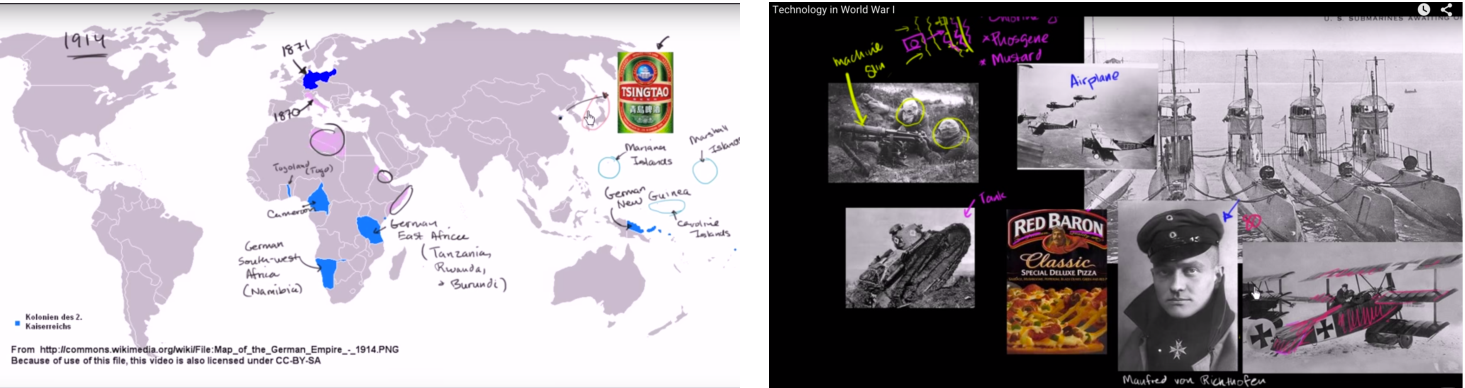
\includegraphics[width=\textwidth]{images/humanities_lec.pdf}
%        \caption{\VEDIT{Our segmentation algorithm assumes that distinct visual entities are more or less separate from each other. For example, a history lecture
%where most of the writing is on top of a map, or where figures are overlayed
%on top of each other (Figure~\ref{fig:humanities_lec}) may require a different method. }}
%        \label{fig:humanities_lec}
%\end{figure}

\subsection{Conclusion}
This chapter introduced \systemname , a readable and interactive representation of blackboard-style lecture videos, which interleaves visual content with corresponding text. We use a variant of the classic line-breaking algorithm to segment the visual content of a lecture video into discrete figures. Then, we leverage the temporal correspondence between the figures and transcript sentences to structure the transcript text. Finally, we interleave the figures with corresponding text in an easy-to-read format. User evaluation suggests that compared to a standard video player and a state-of-the-art interface for watching blackboard-style lectures, users prefer our interface for learning. It also suggests that \systemname\ is effective in helping users browse or search through lecture videos. 

